\chapter{Registration Pipeline using Line Features}
In this chapter we describe how the Vector-valued Gaussian Model is utilized in our implementation of a 3D Face Registration Pipeline. To additionally enhance the registration outcome of this pipeline we use face data where the key regions have been marked with contour lines. In the following we provide a description of line features and their use as well as a specification of the registration pipeline. 
\viscomment{pipeline type important?}

\section{Line Features}
Line features serve the purpose of augmenting the quality of registration by initiating it with a larger set of corresponding points, by sampling points from the lines themselves. They are used to mark complex regions of the face, i.e. the eyes and ears, so that the registration process produces an accurate mapping of the contours of these organs which would otherwise not be possible. Without the prior information provided by line features, an accurate mapping in these
regions is hard to achieve, because they have a dense abundance of points, while regions like the cheeks are scarcely defined by points.\\
\viscomment{the following is some old text ready to incorporate}
The idea behind the use of sampled points from the line features was to have more point correspondencies in complex regions as for example the eyes and the ears where there is a great abundancy of pixels and the algorithm isn’t likely to create a flow field which is accurate not enough to describe these regions, because of it’s smoothness constraint.

For every scan we want to register, we have 8 contours given. These have been marked on three images of every face, see Fig section 1.3, with a special Graphical User Interface for marking points and lines on images. The contours we call line features depict the eyebrows, eyes, ears and lips of a face. They are made up of a set of segments, each of which is modelled with a \textbf{B\'{e}zier curve} of a specified order. B\'{e}zier curves are often used in Computer
Graphics for modelling smooth curves of varying order. Given a set of control points $\mathcal{P} = \{P_{0}, P_{1}, P_{2}, \ldots, P_{n}\}$ the B\'{e}zier curve through these points is given by
\begin{equation}
    C(t)=\sum_{i=0}^{n}P_{i}B_{i,n}(t)
\end{equation}
where $B_{i,n}(t)$ is a Bernstain polynomial 
\begin{equation}
    B_{i,n}(t)=\begin{pmatrix} n \\ \\ i \end{pmatrix}(1-t)^{n-i}t^i
\end{equation}
and $t \in [0,1]$ is the curve parameter. The Bernstein polynomials of degree n form a basis for the power polynomials of degree n. 
Due to the nature of the objects depicted, there are open as well as closed curves. 

\begin{comment}
\def\eyepath{(-3,0) .. controls (-2,1.8) and (2,2.2) .. (2.7,0) .. controls (2,-1.2) and (-2,-1.4) .. (-3,0)--cycle;}
\def\eyebrowpath{(3,0.5) .. controls (3,1.5) and (6.5,1.5) .. (7,0.5) .. controls (5.5,0) and (2,-0.5) .. (4.8,0.5);}

\begin{tikzpicture}
    \draw[black]\eyepath
    \draw[black]\eyebrowpath
\end{tikzpicture}

\viscomment{draw eye and eyebrow with bezier curves, first look at real world recorded images}
\end{comment}

\begin{figure}[h!]
    \centering
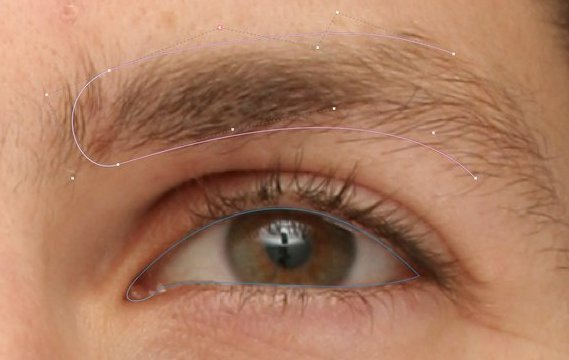
\includegraphics[width=\textwidth]{./resources/img/eyebrow_left.jpeg}
\caption{Line Features of the left eyebrow and eye, consisting of b\'{e}zier curves defined by visible control points (white)}
\end{figure}

\section{Sampling 3D Points from 2D Line Features} 
The line features provide us with additional prior information about the nature of the deformation field. In order to incorporate the line features in the Vector-valued Gaussian Model, we agreed to use them as additional point-wise information. In order to get this point-wise information the line features are sampled at discrete intervals resulting in a set of additional landmarks $L_{Add} = \{l_{1}, \cdots, l_{N}\}$. These
define the mapping $\Omega:L_{Add\mathcal{M}} \rightarrow L_{Add\mathcal{T}}$ of the contours - describing the different important features present in the faces - in the template face mesh on those of the target face mesh. In order for the mapping $\Omega$ to be approximately plausible, we choose an equidistant parametrization. In effect, when a curve is sampled at N points, these N points are all at equal parametric intervals.
\begin{comment}
Bei den Ohren ist die Korrespondenz wirklich schwierig und auch als Mensch je nach Ohrenpaar kaum zu bestimmen. Gerade die Struktur der Ohrmuschel kann wohl nicht immer in korrespondenz gebracht werden. Jedoch sind alle Ohren durch eine äussere Linie begrenzt und die wollen wir matchen. Nun ist es in der Tat so, dass nicht immer alle Ohrläppchen gleich gross sind oder markante Krümungen der äusseren Ohrlinie an der gleichen Stelle auftreten. Wir ignorieren dies jedoch / bzw wir
vereinfachen dies durch unsere Äquidistantz Annahme und sagen dies sei dann genügend gut registriert und störe das Model das wir bauen nicht zu sehr.
\end{comment}
\viscomment{equidistant parametrization is not a fact, it is a choice. Different ears have different topology?}
\def\earpathf{(-1,1.5) .. controls (-1,2.3) and (1,2.8) .. (1,1.5) .. controls (1, -.2) and (0.3,-.1) .. (0.3,-1) .. controls (0.2,-1.5) and (-.5, -1.7) .. (-1,-1.25);}
\def\earpathl{(3,2) .. controls (3,3.3) and (5.6,3.7) .. (5.6,2) .. controls (5.6, 0) and (4.6,0) .. (4.6,-1.3) .. controls (4.6,-2) and (3.5, -2) .. (3,-1.5);}

\begin{figure}[h!]
    \centering
    \begin{tikzpicture}
        \draw[black]\earpathf
        \fill (-1,1.5) circle[radius=2pt];
        \fill (0.1,2.3) circle[radius=2pt];
        \fill (1,1.5) circle[radius=2pt];
        \fill (0.8, 0.25) circle[radius=2pt]; 
        \fill (0.3,-1) circle[radius=2pt];
        \fill (-1,-1.25) circle[radius=2pt];
        \draw[black]\earpathl
        \fill (3,2) circle[radius=2pt];
        \fill (4.3, 3.12) circle[radius=2pt];
        \fill (5.6,2) circle[radius=2pt];
        \fill (5.25,0.35) circle[radius=2pt];
        \fill (4.6,-1.3) circle[radius=2pt];
        \fill (3,-1.5) circle[radius=2pt];
        \draw[ultra thick, blue, ->] (-.8,1.5) -- (2.8,2);
        \draw[ultra thick, blue, ->] (1, 0.25) -- (5.1, 0.35);
        \draw (1.8, .9) node {\Large\textcolor{blue}{$\Omega$}};
        \draw (-1,.5) node {line feature of $\mathcal{M}$};
        \draw (4,1.2) node {line feature of $\mathcal{T}$};
    \end{tikzpicture}
    \label{fig:DiffEars}
    \caption{Mapping of equidistant samples of \textbf{ear} line features from the reference (left) on to the target (right)}
\end{figure}

\subsection{Arc Length Parametrization}
The first problem which becomes apparent when trying to sample the line features is that the b\'{e}zier curve segments don't allow for equidistant parametrization, because the underlying parameter $t \in \mathbb{R}$ is not linear in respect to the length of the curve. The growth of the parameter of a b\'{e}zier curve is instead dictated by velocity.

\def\earpathf{(-1,1.5) .. controls (-1,2.3) and (1,2.8) .. (1,1.5) .. controls (1, -.2) and (0.3,-.1) .. (0.3,-1) .. controls (0.2,-1.5) and (-.5, -1.7) .. (-1,-1.25);}
\def\earpaths{(3,1.5) .. controls (3,2.3) and (5,2.8) .. (5,1.5) .. controls (5, -.2) and (4.3,-.1) .. (4.3,-1) .. controls (4.2,-1.5) and (3.5, -1.7) .. (3,-1.25);}
\begin{figure}[h!]
    \centering
    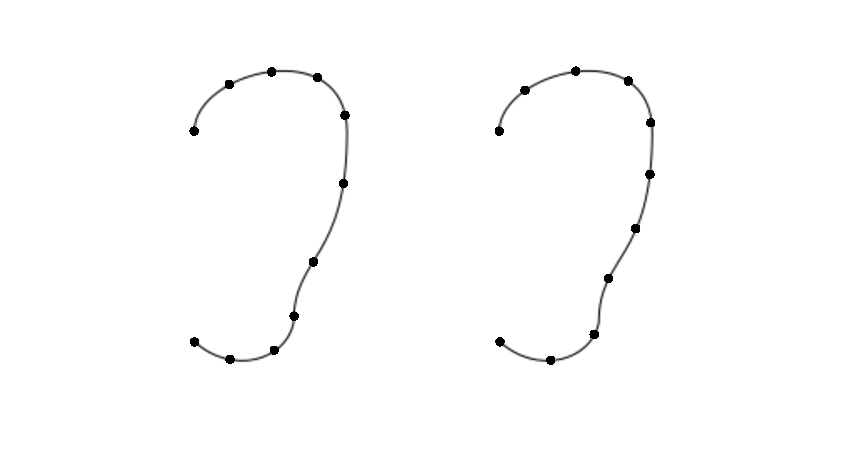
\includegraphics{./resources/figures/ears_diffparam.eps}
    \label{fig:diffparam}
    \caption{a simplified - the depicted \textbf{ear} line feature is treated as one sole b\'{e}zier segment - illustration of the difference between b\'{e}zier (\textbf{left}) and equidistant (\textbf{right}) parametrization.}
    \begin{comment}
    \begin{tikzpicture}
        \draw[black]\earpathf
        \draw[black]\earpaths
        \fill (-1,1.5) circle[radius=2pt];
        \fill (0.1,2.3) circle[radius=2pt];
        \fill (1,1.5) circle[radius=2pt];
        \fill (0.8, 0.25) circle[radius=2pt]; 
        \fill (0.3,-1) circle[radius=2pt];
        \fill (-1,-1.25) circle[radius=2pt];

        \fill (3,1.5) circle[radius=2pt];   
        \fill (3.3,2) circle[radius=2pt];
        \fill (4.1, 2.3) circle[radius=2pt];
        \fill (4.85, 2) circle[radius=2pt];
        \fill (4.99, 1.4) circle[radius=2pt];
        \fill (4.85, 0.4) circle[radius=2pt];
        \fill (4.4, -.45) circle[radius=2pt]; 
        \fill (4.3, -1.05) circle[radius=2pt]; 
        \fill (3.9, -1.45) circle[radius=2pt]; 
        \fill (3,-1.25) circle[radius=2pt];
    \end{tikzpicture}
    \end{comment}
\end{figure}
Consequently, the imperative must be instead to evaluate the curves based on their arc-length, which is defined as the length of the rectified curve. The underlying parameter must then correspond - at every point of the curve - to the ratio between the length of the part of the curve that has been traversed and the total curve length.

\paragraph{In theory}
It is possible to get the arc length $L(t)=\int_{t_{0}}^{t_{1}} \left|C'(t)\right| dt$ for given parameters $t_{0}, t_{1}$ where $C'(t)$ is the derivative of the curve $C:t \in [0,1] \rightarrow \mathbb{R}^2$. We, however, want to find a reverse mapping from the length of a fraction of the curve to the curve parameter $t = L^{-1}(l)$. 
This mapping can of course be derived analytically, but it is far easier to implement it using a numeric approximation. 

\paragraph{In practice}
As we are not in need of a subpixel resolution, we can skip the formal math and use a lookup table to compute the arc-length.
First, we calculate a large number of points on each segment of the curve using the parametrization of the corresponding b\'{e}zier curve. For each point we save its approximate distance from the origin of the segment as a key into a new slot in the lookup table of this segment, while its coordinates act as the slot value. 
\begin{figure}[h!]
\centering
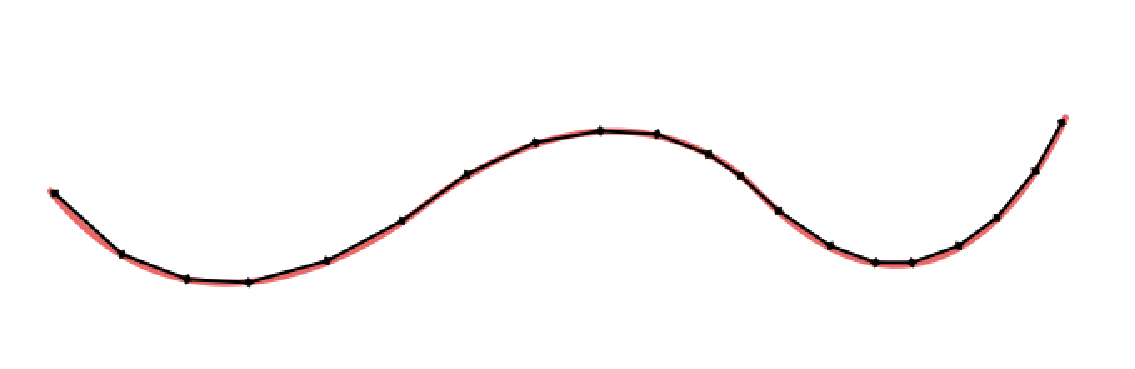
\includegraphics[width=\textwidth]{./resources/figures/lookup_table.eps}
\label{fig:lookup}
\caption{Visualization of euclidean distances between points computed with b\'{e}zier curve parametrization. This is an arbitrary line feature used solely for demonstration purposes.}
\end{figure}
The distance is approximated by summing up the euclidean distances of each point to its respective predecessor starting from the origin.

The resulting lookup table contains the approximative distances and coordinates of a large number of points from the origin of a curve segment. Assembling the segments' lookup tables gives us the table table for the whole curve with the last key representing its arc-length.\\ 
Second, the curve can now easily be sampled by computing the length of parametric intervals $\frac{L}{N}$ for a specified number of points N. $l=k \cdot \frac{L}{N}$ returns the current length of the curve for the sampling point of index k, where $k=[0,\cdots,N]$ for open curves and $k=[0,\cdots,N-1]$ for closed curves.
To get the point coordinates for a fraction of the curve we now simply perform a binary search on the lookup table for this distance. We choose index which returns the coordinates for the exact fraction length and if that is not the case the index with the next smaller length. The coordinates of the point either exactly or approximately computed for the given fraction length of the curve is used as the sampled point.

\subsection{3D Mesh Projection of Sampled Points}
Having implemented arc length parametrization it is possible to draw an arbitrary amount of samples $x \in \mathbb{R}^2$ from the line features. They are then defined as a set of points $S \subset \mathbb{R}^2$. Our goal is, however, to have these additional landmarks describing the features on the mesh of a face itself and not a 2-dimensional snapshot thereof.
Because we have no information on the depth of the line features, we have to project the sampled points of each line feature onto a face mesh in order to obtain their approximate 3D representation. 
\viscomment{Introduce camera model with schema here?}
In the camera model the image is located on the viewing plane or viewport opposite of the focal point. (computes 3D direction of 2D sample point)
The direction of the 3D representation of a point on a curve is given by the (normalized) vector defining the position of the point on the viewing plane from the perspective of the focal point of the camera.
Given: diskrete mesh, how to choose point?
We now a seek a mesh vertex that is the most accurate representation of a sample point on the 2D curve. The dot product of their normalized directions is used as a similarity measure. In order to find a corresponding vertex, we save all the distances of mesh vertices in a list which have a similarity measure that is higher than a specified threshold. We then select the distance of the vertex with the maximum similarity.
Finally, we project the distance of this vertex onto the direction of our sample point and thereby obtain an approximation of the points position in the mesh.
%\begin{wrapfigure}[]{o}[2cm]{\documentwidth}
\begin{figure}[h!]
    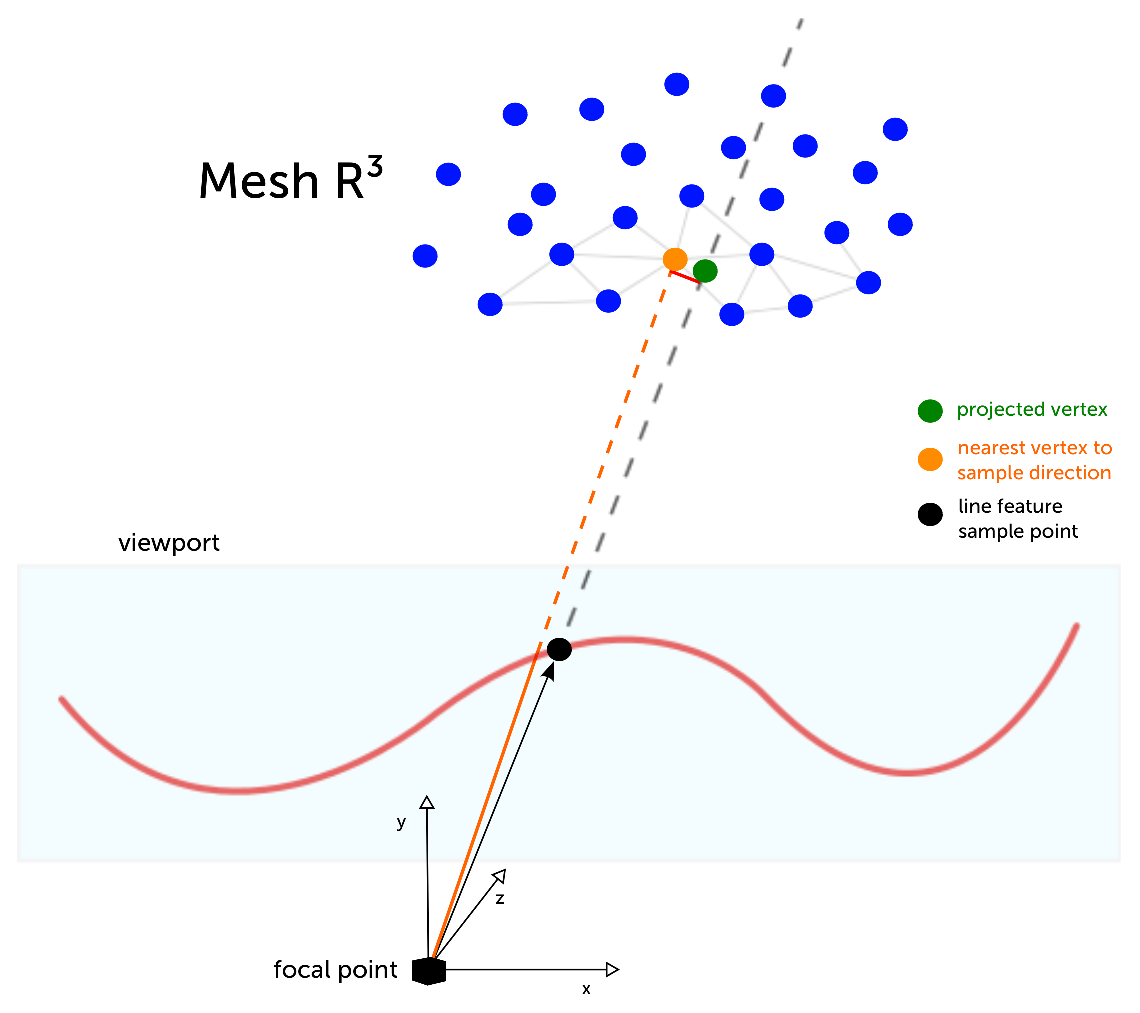
\includegraphics[width=\textwidth]{./resources/figures/projection.eps}
\label{fig:projectio}
\caption{shows the projection of a sample point - on a 2D line feature - from the viewport onto a triangulated 3D mesh. The distance vector of the vertex with the most similar direction vector (orange) is projected (red) onto the direction of the sample point (black arrow), resulting in the projected vertex (green)}
\end{figure}
\paragraph{Problems \& Inacurracies}
The face meshs used in the face registration pipeline contain large holes around the ears and the eyes. In effect, the projected sample points are off target, because now the mesh vertex with the most similar direction is likely farther away at a suboptimal location. This circumstance leads to the projected line not clearly being distinguishable as a contour line. On different data sets the performance of the projection of the line features for a large number of
samples, i.e. 30, varied significantly. Overall one can say that the distortion of a projected line increases with the amount of sample points.
\viscomment{Compute some landmarks with 30 samples}
\viscomment{up close image of eye holes of face scan}
An easy workaround was to reduce the number/amount of sample points. By using only 5-10 sample points per curve some datasets rendered near perfect results on a ``control dataset''. \viscomment{Compile list of datasets, show samples} 
However, when the holes are too large this workaround also fails. This circumstance leaves room for discussion. As long as the method is dependent on the data from the scans - the size of the holes in the meshs - it lacks generality and generality is exactly the basis for feasible and reproducable registration results.\\

\paragraph{Preparing the Template Mesh}
In the next step, the line features also had to be marked on the template mesh. As the template mesh we use the mean mesh of the 3DMM of the Graphics and Computer Vision Group at the University of Basel. In order to mark the features, the mean mesh first had to be rendered with three different camera callibrations. The 2D line features where then projected back onto the mesh using these callibration parameters. The mean mesh already had 60 feature points
clicked manually, many of which were not added to the face scans.
\begin{comment}
In the previously used registration method, a large number of points was used for each curve. These points were, however, not projected directly on to the 3/4 shells of the mesh. Instead their location was constrained by computing a 1-dimensional band of points before and after their approximate position, seen from the origin.
then a band of points is computed perpendicular to the line along the direction at each computed point that cuts through the mesh and serves as a horizontal constraint for the points to lie after the registration.
so that if 
Because of global angle comparisons between the direction from the camera towards the vertices and the direction towards the projection of a sampled point on the line
if there is a hole in the mesh at the destination of this direction vector on the mesh and the direction of vertex is used can be used which actually distorts the shape of line
\end{comment}

After the projetion, we have added samples from the line features to our set of landmarks. We therefore have provided the registration algorithm with additional prior information to define the deformation field by and to produce a better fitting result.

\section{Rigid Mesh Alignment}
Before we can start with initializing Gaussian Models, we first have to ensure that template and target mesh are aligned in the same coordinate system. After all, we want to model the variability of different faces without incorporating an additional offset. We therefore have to perform a rigid transformation \viscomment{What kind of RT?} 
rotation + translation
% http://www.math2k.com/pre-algebra/rigid-transformations-examples-and-worksheets/
aligning the meshs according to their landmarks. \viscomment{Now in order to receive a perfect mapping of the floating mesh on to the mean/reference mesh we have to allow for 3 degrees of freedom, that is in all 3 dimensions x,y and z, for every pixel in the floating mesh except for the reference points we have used as correspondencies. The parameters having the most influence to the mapping will be those specified in the constraints we introduced into the equation via
regularization.} We use the set of landmark whose identifiers are present in both meshs.
\viscomment{The face scans have to be clipped at the neck and around the ears where the scanner has left artifacts.} 
The computed transformation is applied to all vertices of the respective face scan. 
The mean face was broader in shape than the scan and was perfectly coated in texture for the simple reason that hours of manual labour have been invested to render this important piece of data a perfect reference.
\viscomment{Show 3 images of overlap of mean with different scans}
The aligned meshs serve as the starting point for the registration.

\begin{figure}[h!]
\centering
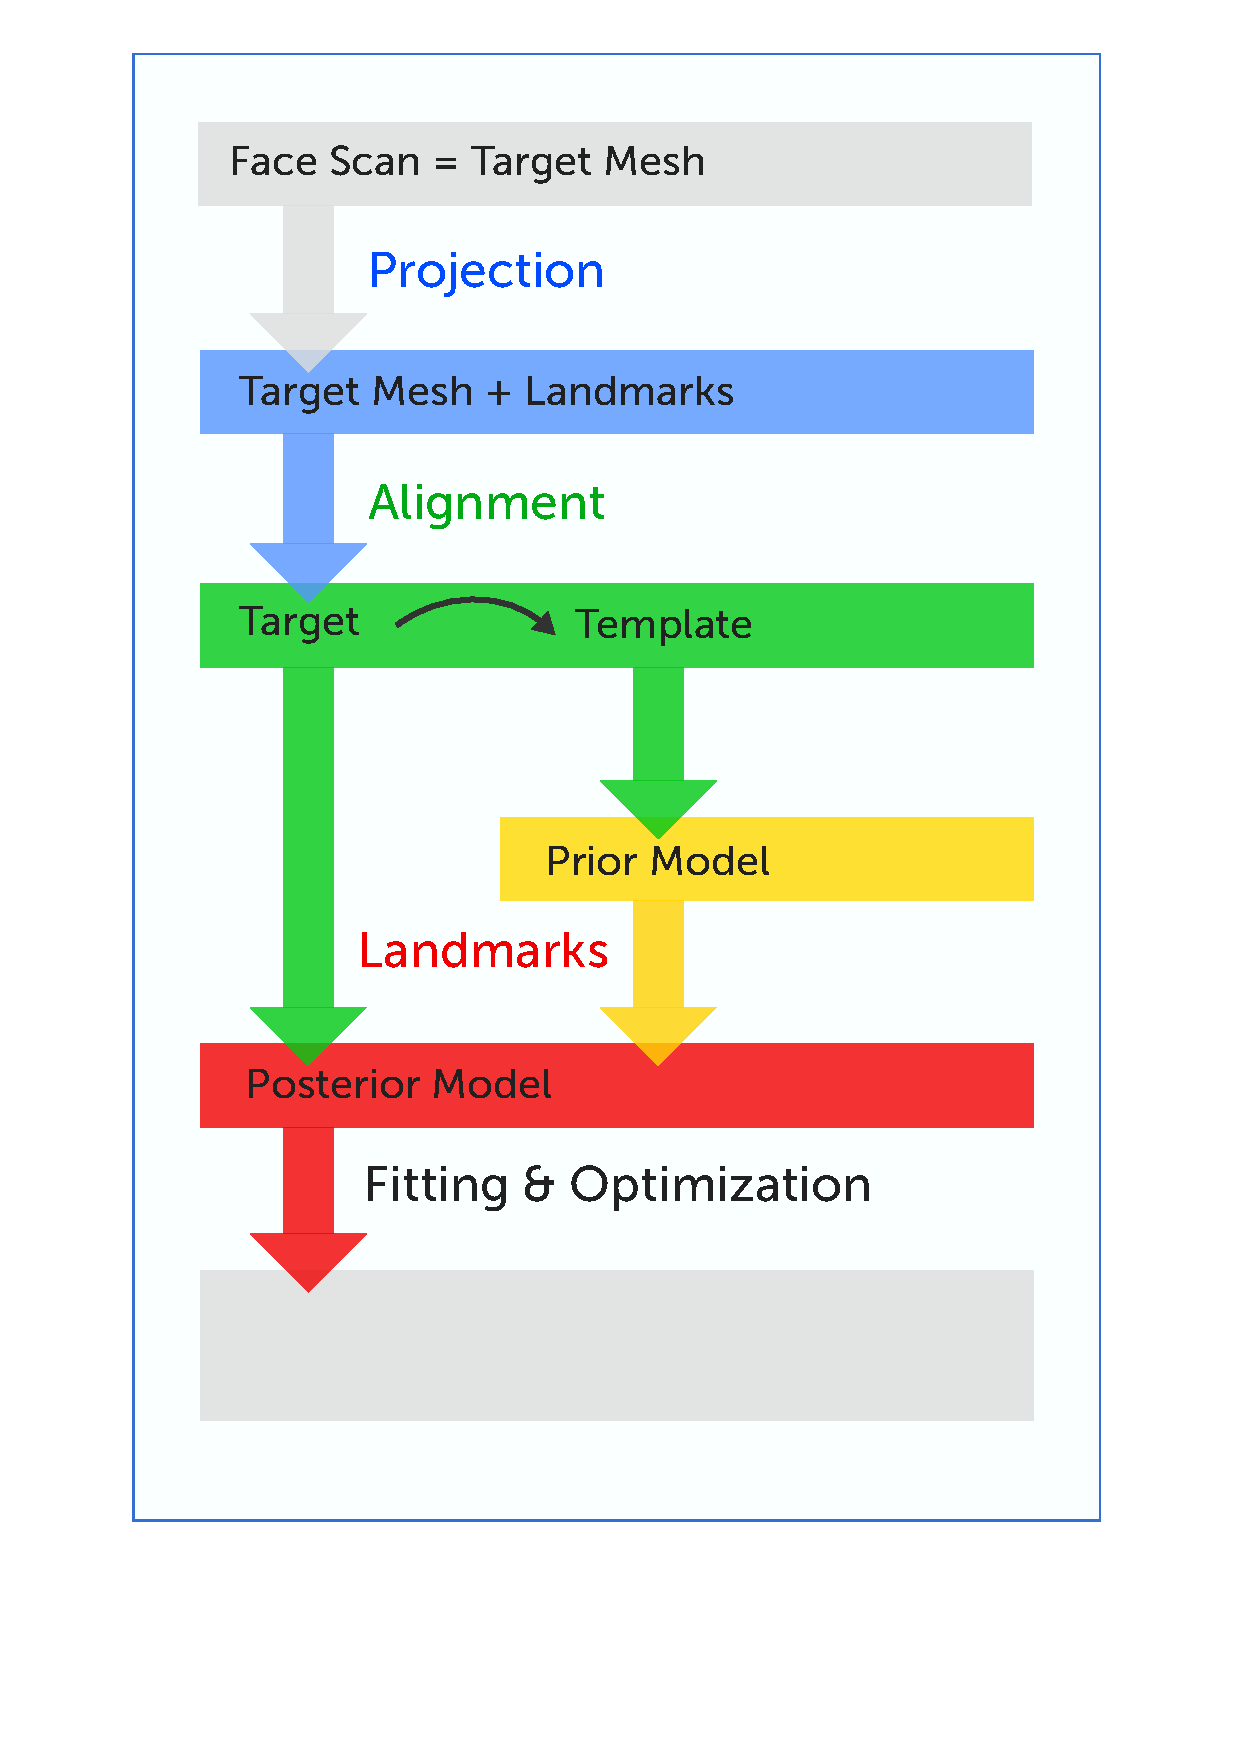
\includegraphics[width=\textwidth]{./resources/figures/pipeline.pdf}
\label{fig:pipeline}
\vspace{-90pt}
\caption{Fitting pipeline: blablabla}
\end{figure}

We are now set for the actual registration involving the Prior and Posterior Gaussian Models and the Fitting. For the definition of the Gaussian Process distributions we use the software framework statismo developed at the Computer Science Department of the University of Basel. It is a framework for PCA based statistical models. These are used to describe the variability of an object within a population, learned from a set of training samples. We use it to generate a
statistical model of the template mesh. Furthermore we use the software package gpfitting for the actual fitting. 

\section{Prior Model}
imperative: build prior faces resulting from possible deformations of template
The Gaussian Process Prior distribution of the template mesh is represented as an object and the parameters are saved on to disk. This allows for samples to be drawn from this representation of the Gaussian Process Prior Model. These samples are 3D face mesh that are the result of the deformations generated by the Gaussian Process Prior and then added to the template mesh. They are examples for possible deformations defined solely on the ground of the covariance of the template mesh points.
\viscomment{show some examples here, or already in chapter 3}

\section{Posterior Model}
imperative: build posterior model from combination of the prior model and the target landmarks. \viscomment{Landmarks are added to the distribution as additional points and co-define the deformation for the mesh vertices}
Build Model from mean and target landmarks. This time we incorporate the mapping information of the landmarks and get a model where the
We get valid face like meshs for different deformations, which are fixed at the target landmarks.

\section{Fitting}
Perform optimization
Show some fits?

What are we optimizing? L2??? --> not robust to outliers, protruding regions.
\section{Robust Loss Functions}\viscomment{Optimizing the loss function?}
After the alignment of template and target mesh, the template protrudes over the target on the upper side of the head and the side of the neck.
\viscomment{show an image with template and target on top of each other}
Performing optimization as described in \ref{sec:optimization} using a simple Mean Square Error(MSE) as a distance measure between the template and target mesh penalizes the portruding regions of the template with a strong gradient towards the rims of the template and therefore causes strong distortions. 
\viscomment{show image of failed fitting, next to target}

Our approach to tackling this problem was to try out a range of different robust estimators, namely the Tukey, Huber, and Fair estimators. The advantage of these
estimators lies therein that they are less sensitive to outliers, reducing registration artifacts considerably. (Outliers are in this case template mesh points that farther away than a certain threshold from the next point on the target mesh} However, as can be seen from the formulas, these techniques require finding appropriate parameters first which produce reasonable/acceptable visual results.

Fair
\begin{subequations}
\begin{equation}
\rho(x)=c^2\left[\frac{\left|x\right|}{c}-log(1+\frac{\left|x\right|}{c})\right]
\end{equation}
\begin{equation}
    \psi(x)=\frac{x}{1+\frac{\left|x\right|}{c}}}
\end{equation}
\end{subequations}
Huber
\begin{subequations}
\begin{equation}
    \rho(x) = \twopartdef {\frac{x^2}{2}} {\left|x\right|<k} {k(\left|x\right|-\frac{k}{2})} {\left|x\right|\geq k}
\end{equation}
\begin{equation}
    \psi(x) = \twopartdef {x} {} {k sgn(x)}{} 
\end{equation}
\end{subequations}
Tukey
\begin{subequations}
\begin{equation}
    \rho(x) = \twopartdef {\frac{c^2}{6}\left(1-\left[1-\left(\frac{x}{c}\right)^2\right]^3\right)} {\left|x\right|\leq c} {\frac{c^2}{6}} {\left|x\right| > c}
\end{equation}
\begin{equation}
    \psi(x) = \twopartdef {x\left[1-\left(\frac{x}{c}\right)^2\right]^2} {} {0} {}
\end{equation}
\end{subequations}
\viscomment{for each estimator show a sequence of fits for different parameters and 3 different meshs?}

\section{Varying the Variances}
